\documentclass[10pt,a4paper]{article}
\usepackage[utf8]{inputenc}
\usepackage[italian]{babel}
\usepackage{amsmath}
\usepackage{amsfonts}
\usepackage{amssymb}
\usepackage{graphicx}
\usepackage[left=2cm,right=2cm,top=2cm,bottom=2cm]{geometry}
\newcommand{\rem}[1]{[\emph{#1}]}

\author{Gruppo BN \\ Federico Belliardo, Marco Costa, Lisa Bedini}
\title{Ottica 2}
\begin{document}

\maketitle
\section{Scopo dell'esperienza}
L'esperienza si divide in due parti distinte. Nella prima si stima la lunghezza d'onda della radiazione di un laser a diodo mediante la misura degli ordini di diffrazione provocati dall'incidenza sulla scala graduata di un calibro utilizzata come reticolo. Nella seconda parte mediante un laser He-Ne si calibra un interferometro di Michelson per eseguire la misura della lunghezza d'onda della riga verde del mercurio, e in seguito osservare le frange di interferenza con luce bianca.

\section{Materiale occorrente}
\begin{itemize}
\item Calibro;
\item Laser a diodo;
\item Metro a nastro;
\item Interferometro di Michelson;
\item Laser He-Ne;
\item Lampada al mercurio;
\item Lampada a luce bianca;
\item Filtro verde;
\end{itemize}

\section{Parte A - Misura della lunghezza d'onda del laser a diodo}
\subsection{Modalità operative}

\begin{figure}[!htb]
  \centering
  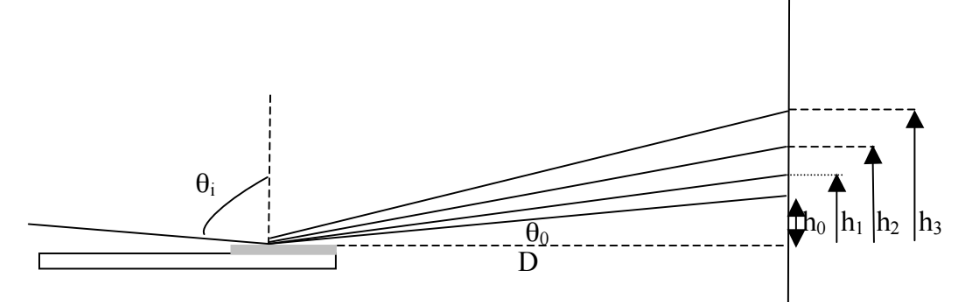
\includegraphics[scale=.5]{disegno1.png}
\caption{Disegno schematico dell'esperimento di diffrazione.}
\label{parteAfigura}

\end{figure}
La spaziatura tra le suddivisioni della scala graduata del calibro è troppo grande per poter essere usata come reticolo di diffrazione per la luce visibile senza l'accorgimento di far incidere il fascio in modo radente alla scala, cioè con angolo di incidenza prossimo a $\frac{\pi}{2}$. Il fascio riflesso e i vari ordini di diffrazione sono visibili un un muro (schermo) a circa due metri di distanza.\\
Sul muro si è posto un foglio di carta su cui si sono segnati il punto in cui il laser sarebbe arrivato se non fosse stato diffratto\footnote{Infatti, essendo l'angolo inferiore a $\pi /2$, una parte di fascio non viene diffratta.}, il punto in cui il fascio viene riflesso dal calibro e i vari ordini di diffrazione dal calibro. La media delle posizioni del punto di incidenza diretta e del punto di riflessione è la proiezione del piano del tavolo proiettato sul muro. Da questo punto è necessario misurare la distanza $D$ (distanza tra il calibro e il muro) e tutte le lunghezze $h_0, h_1, h_2,...$. indicate nella figura \ref{parteAfigura}.\\
Per praticità si è fatto incidere il fascio laser su uno specchio fisso sul tavolo prima di farlo giungere al reticolo di diffrazione.\\ 
%Inserire altri eventuali accorgimenti sperimentali su come si misurano d e D e %dire come sono stati presi gli errori su queste misure.\\
Il fascio laser incide su una vasta parte della scala graduata generando una macchia luminosa oblunga sul calibro. Come punto da cui misurare $D$ si è preso dal muro alla fine del calibro.\\

%Forse sarebbe meglio prendere la media tra l'inizio e la fine del fascio sul calibro per la stima di D?

%FIXME - MARCO COSTA: Spiegare perchè la componente principale del fascio è data dalla rifrazione sulla fine del calibro.

\subsection{Raccolta ed elaborazione dati}

L'incertezza sulla misura delle posizioni dei minimi di diffrazione è stata presa come il massimo tra l'ampiezza della riga luminosa diffratta e la tacca del metro a nastro ($0.5 \,mm$). L'incertezza su $D = 204.4 \pm 0.5 \, cm$ è una stima che tiene in considerazione l'incertezza nel posizionamento delle estremità del metro e la sua curvatura lungo il percorso, mentre per $d$ si è preso il valore nominale della separazione delle tacche della scala graduata del nonio dunque $d = 1.00 \pm 0.01 \, mm$. L'incertezza su quest'ultima misura è una stima sulla precisione meccanica di realizzazione delle tacche.\\
%Ho paura che questo errore sia troppo garnde Podo lo scrive molto più piccolo.
La legge del reticolo per questa configurazione geometrica è: $d(\sin  \theta_i - \sin \theta_d)  = m \lambda $, dove $\theta_d = \frac{\pi}{2} - \sin \theta_n $. Riscrivendo la legge come: $\sin \theta_d = -m \frac{\lambda}{d} + \sin \theta_i$. La relazione funzionale tra $\sin  \theta_d$ e $m$ è una retta, si è pertanto eseguito un fit dei dati riportati in tabella \ref{Ordini}. Per eseguire il fit si è usata la funzione \emph{curvefit} della libreria \emph{pylab} con l'opzione \emph{$absolute\,sigma = "true"$}. Il fit della funzione lineare $y = ax+b$ ha riportato i seguenti valori: \\

\begin{table}[!htb]
\centering
\begin{tabular}{|c|c|c|}
\hline
Ordine & $h (cm)$ & $ \Delta h$ \\
\hline
0	&	13.0	&	0.2\\
1	&	16.3	&	0.1\\
2	&	18.7	&	0.1\\
3	&	20.8	&	0.1\\
4	&	22.5	&	0.1\\
5	&	24.1	&	0.1\\
6	&	25.6	&	0.1\\
7	&	26.9	&	0.1\\
8	&	28.3	&	0.1\\
9	&	29.5	&	0.1\\
10	&	30.6	&	0.1\\
11	&	31.8	&	0.1\\
12	&	32.8	&	0.1\\
13	&	33.8	&	0.1\\
14	&	34.7	&	0.1\\
15	&	35.6	&	0.1\\
16	&	36.7	&	0.1\\
17	&	37.6	&	0.1\\
18	&	38.4	&	0.1\\
29	&	39.3	&	0.1\\
20	&	40.1	&	0.1\\
21	&	40.9	&	0.1\\
22	&	41.7	&	0.1\\
23	&	42.5	&	0.1\\
24	&	43.3	&	0.1\\
25	&	44.0	&	0.1\\
26	&	44.7	&	0.1\\
27	&	45.5	&	0.1\\
28	&	46.4	&	0.1\\
\hline
\end{tabular}
\caption{Ordini di interferenza e relativa altezza dal piano del tavolo.}
\label{Ordini}
\end{table}

Le distanze riportate in tabella \ref{Ordini} indicata sopra sono riferite al punto in cui il fascio indisturbato colpisce al muro. Esse vanno riscalate per il punto zero che è il punto medio tra quello detto e il punto di riflessione (cioè l'ordine 0).\\

Nella figura \ref{interferenza} sono riportati i dati e il fit lineare con retta $y = ax+b$, l'algoritmo di minimizzazione del $\chi^2$ fornisce: $a = ( -6.37 \pm 0.02 ) \cdot 10^{-4}$, $b = 0.994 \pm 0.002$; la matrice di covarianza è:\\ $ \Sigma_{ij} = \left( \begin{array}{cc}
5.54 \cdot 10^{-12} & -2.93 \cdot 10^{-11} \\ 
-2.93 \cdot 10^{-11} & 3.85 \cdot 10^{-10}\\
\end{array} \right)$. Con un $\chi^2/ndof = 2/27 \, (ndof)$.\\
Il $\chi^2$ ottenuto è molto piccolo, ciò significa che nella differenza eseguita tra i dati riportati in tabella e il punto di riferimento citato più volte la propagazione corretta degli errori ha sovrastimato le incertezze.\\

%Dire se consideriamo più spesso errori statistici o errori massimi e come si sono propagati anche in relazione a absolute sigma.

\begin{figure}[!htb]
  \centering
  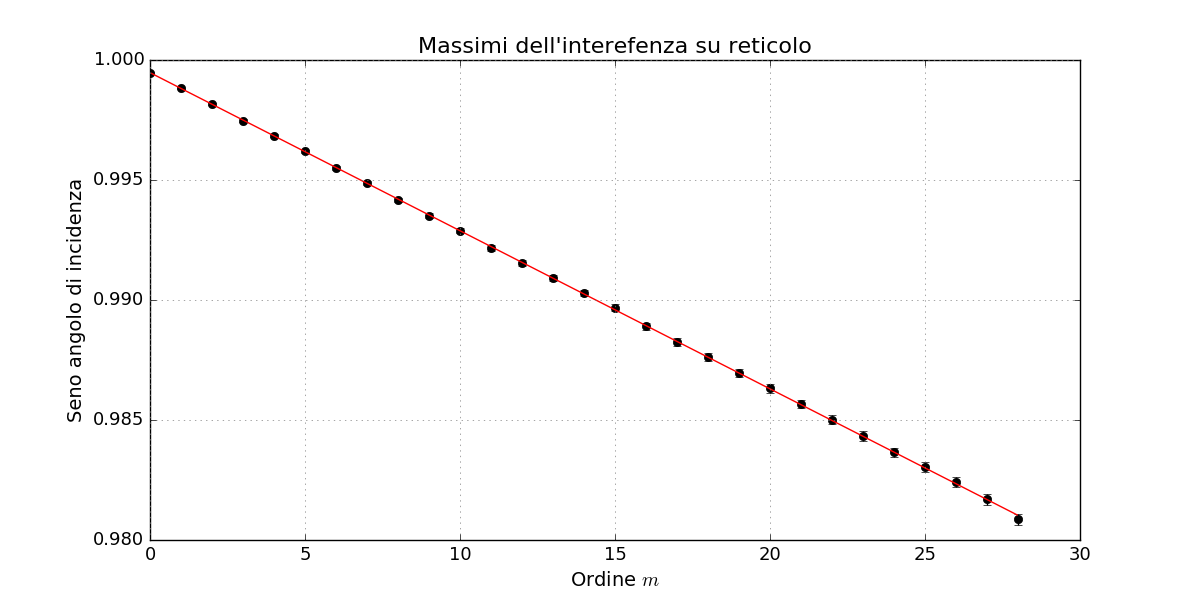
\includegraphics[scale=.5]{plot.png}
\caption{Seno dell'angolo di interferenza in funzione dell'ordine.}
\label{interferenza}
\end{figure}

%Errore troppo grande dovuto a scelta di errore su d
Dal parametro $a$ si ricava il valore di $\lambda = 638 \pm 7 \, nm$ da confrontare con quello teorico del laser $\lambda = 636.3 \, nm$, i due valori sono perfettamente compatibili. L'errore della misura è dovuto alla sovrastima dell'incertezza sull'errore si costruzione della scala graduata del calibro. E' anche possibile le le differenze statistiche sulla lunghezza delle tacche si si medino a zero nell'interferenza per dare un contributo effettivo all'incertezza drasticamente ridotto.\\

\section{Parte B - Misura della lunghezza d'onda della riga verde del mercurio}
\subsection{Calibrazione interferometro}

\begin{figure}[!htb]
  \centering
  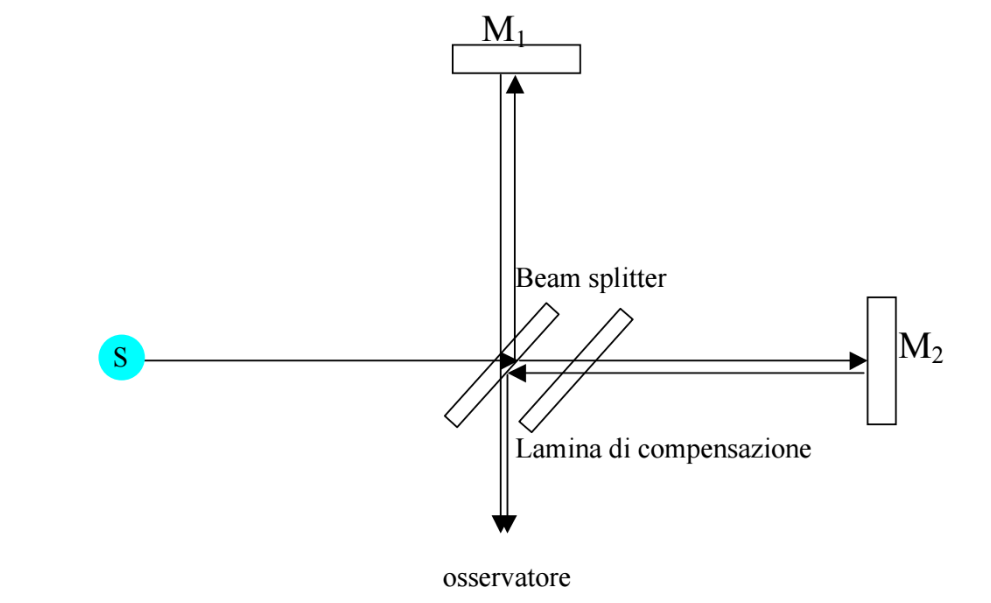
\includegraphics[scale=.5]{interferometro.png}
\caption{Disegno schematico dell'interferometro di Michelson.}
\label{int}
\end{figure}

L'interferometro di Michelson in dotazione è dotato di una vite che permette di spostare l'orientazione dello specchio $M2$ (vedi figura \ref{int}) e di una vte micrometrica dal passo di $10 \, \mu m$ e fattore di demoltiplica ignoto che permette di spostare lo specchio $M1$. E' necessario prima misurare quale sia il rapporto tra il passo della vite e lo spostamento effettivo dello specchio, cioè misurare il fattore di demoltiplica della leva. \\
Per fare ciò si utilizza una sorgente laser He-Ne di lunghezza d'onda nota e si misura lo spostamento della vite necessario perché $N$ frange passino per un certo punto dello schermo. \\
Dalla formula $2 \Delta X = m \lambda$ si è ricavato $\Delta X$ e quindi il fattore di demoltiplica $\eta = \frac{\Delta X}{\Delta s}$, dove $\Delta s$ è lo spostamento letto sulla vite micrometrica.\\
Per contare più agilmente le frange si sono ripresi alcuni video della figura di interferenza per vari $\Delta s$ della vite. Si è scelto il video migliore, corrispondente a $\Delta s = 200 \pm 5 \, \mu $ \footnote{L'incertezza su $\Delta s$ è stata assunta essere mezza tacca della vite cioè $5 \, \mu$, così facendo la si è probabilmente molto sovrastimata.} e si sono effettuati conteggi indipendenti che hanno dato come risultato la media: $N = 125 \pm 5$, dove la media è la semidispersione massima. Dalle precedenti formule $\eta = 5.0 \pm 0.2$. L'errore sulla misura di $N$ è da intendersi di natura statistica nonostante il modo con cui sia stato stimato causa le poche misure.\\
Una della principali difficoltà di misura è stato il leggero ritorno della vite micrometrica.\\

\subsection{Misura di lunghezza d'onda}
Si è cambiata la sorgente luminosa, si è inserita la lampada al mercurio al posto del laser He-Ne, si è aspettato il tempo sufficiente perché ci fosse termalizzazione e si è inserito il filtro verde per selezionare la riga del colore voluto. Si è riallineato il fascio in modo che la figura di interferenza fosse centrale e si è inserita davanti alla sorgente una punta metallica indicatrice per eseguire più facilmente i conteggi. A causa della debolezza del fascio i conteggi sono stati eseguiti a occhio (era impossibile proiettare su uno schermo).\\
Si è presa una misura nel numero di massimi e minimi che si osservano per una variazione $\Delta s = 200 \pm 5$, $N = 150 \pm 5$, la stessa misura è stata eseguita dai tre componenti del gruppo e gli errori riportati sono le semidispersioni delle tre misure eseguite. La lunghezza d'onda misurata risulta essere: $\lambda_Hg = 530 \pm 20$. L'errore grande è dovuto all'errore sulla misura  di $\Delta s$ che è stata sovrastimata.\\


\section{Interferenza di luce bianca}
Inserendo il separatore aggiuntivo è possibile osservare l'interferenza di luce bianca quando i bracci dell'interferometro sono uguali. Questo perché indipendentemente dalla lunghezza d'onda la condizione di interferenza costruttiva è realizzata (è chiaro che una condizione di interferenza distruttiva non può essere realizzata), per quanto detto la diffrazione delle componenti monocromatiche mostra una grande macchia bianca al centro e corone di luce multicolore allontanandosi dal centro.\\ 


Le misure riportate sono state eseguite dai diversi componenti del gruppo, a fianco sono riportati i valori di $\lambda$ calcolati. La media è $\lambda_Hg = $

%Attenzione: non c'è alcuna speranaza di far tornare giuste le lunghezze d'onda -- vedi quello che stampa il file calibrazione.py


\end{document}
